\chapter{Semantica Lessicale}

\section{Introduzione}

\subsection{Programma della Seconda Parte del Corso}

Per quanto riguarda questa parte del corso ci si concentrerà sulla semantica lessicale, in particolare sui seguenti punti:

\begin{itemize}
  \item Problema della Knowledge Representation. 
  \item WordNet e BabelNet. 
  \item FrameNet. 
  \item N-grams. 
  \item Word/Sense embeddings. 
  \item Encoder/Decoder.
\end{itemize}

\subsection{Che cos'è la semantica lessicale?}

\dfn{Semantica Lessicale}{La semantica lessicale è lo studio  del significato delle parole e delle loro relazioni. Lo studio di cosa i singoli oggetti lessicali significano, cosa fanno, come possono essere rappresentati e combinati.}

\paragraph{Sono scelte le ontologie per:}

\begin{itemize}
  \item \fancyglitter{Parte metodologica:} adottare un piano molto interdisciplinare a un alto livello di generalità. 
  \item \fancyglitter{Parte architetturale:} centralità del ruolo che un'ontologia può giocare in un sistema informativo.
\end{itemize}

\paragraph{Le parole sono flessibili:}

\begin{itemize}
  \item Capacità di ripetere le parole nei \fancyglitter{sensi} già noti, combinarle in enunciati anche nuovi, capacità di estendere una parola o una frase per esprimere nuovi sensi: 
    \begin{itemize}
      \item Queste capacità sono ereditate dagli esseri umani. 
      \item Non si sviluppano in ogni circostanza. 
    \end{itemize} 
  \item La cooperazione tra le capacità del punto precedente è importante per sviluppare la \fancyglitter{metalinguistica}:
    \begin{itemize}
      \item Che cosa significa questa parola? Che cosa vuol dire? Si può dire così? Si scrive goccie o gocce? 
      \item Le parole hanno funzione riflessiva: si usa la \fancyglitter{lingua per riflettere sulla lingua}. 
    \end{itemize}
\end{itemize}

\paragraph{Rigidità vs. Deformabilità:}

\begin{itemize}
  \item La chimica e la matematica parlano di determinati aspetti dell'esperienza (sono \fancyglitter{rigide}). 
  \item Le lingue invece sono \fancyglitter{deformabili}: se ne può alterare o dilatare il significato.
\end{itemize}

\subsection{Alcune Definizioni di Ontologia}

\qs{}{Cosa significa il termine ontologia?}

\dfn{Ontologia Filosofica}{
  In filosofia il termine ontologia indica lo studio dell'essere e delle sue categorie fondamentali. Un'ontologia definisce un insieme di primitive rappresentazionali con il quale modellare un dominio di conoscenza o di discorso. È un sistema organizzato in categorie e relazioni. Le loro definizioni includo informazioni sul loro significato e vincoli su come applicarle in maniera consistente.
}

\nt{Per esempio una categoria rappresenta tutti i tipi di entità che possono fungere da soggetto in un predicato.}

\paragraph{Problema:} questa definizione ammette che quasi tutto può essere considerato un'ontologia.

\dfn{Ontologia come Concettualizzazione}{
Un'ontologia è una specifica esplicità di una concettualizzazione. Una struttura formale di un pezzo della realtà come percepito e organizzato da un agente indipendentemente da: 
\begin{itemize}
  \item Vocabolario utilizzato. 
  \item L'occorrenza in una situazione specifica.
\end{itemize}
}

\nt{Situazioni diverse coinvolgenti lo stesso oggetto descritte da un vocabolario diverso possono avere la stessa concettualizzazione.}

\paragraph{Ontologia e semantica:}

\begin{itemize}
  \item Un'ontologia riguarda ciò che c'è, la semantica si riferisce a ciò che c'è. 
  \item Differenti aspetti del linguaggio hanno differenti ruoli nell'ontologia.
\end{itemize}

\paragraph{Ontologie e Knowledge Bases:}

\begin{itemize}
  \item Componente \fancyglitter{terminologica} (ontologia):
    \begin{itemize}
      \item Indipendente da un particolare stato. 
      \item Pensata per supportare servizi terminologici.
    \end{itemize}
  \item Componente \fancyglitter{asserzionale}:
    \begin{itemize}
      \item Riflette specifici stati. 
      \item Pensata per problem solving.
    \end{itemize}
\end{itemize}

\begin{figure}[h]
    \centering
    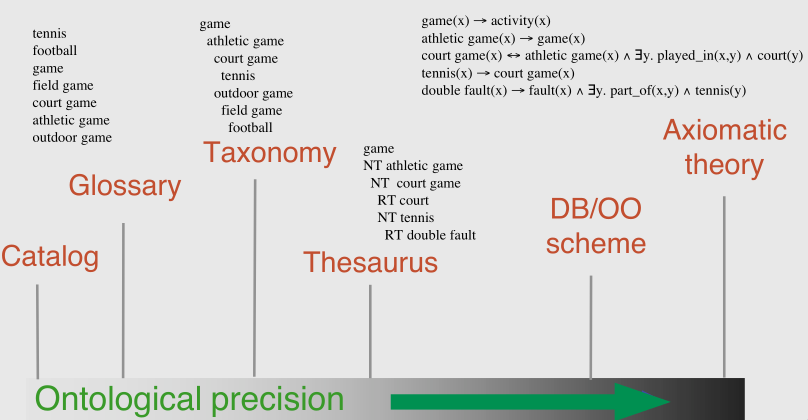
\includegraphics[scale=0.5]{01/precision.png}
    \caption{Livelli di precisione delle ontologie.}
\end{figure}

\paragraph{Ontologia e lessico:}

\begin{itemize}
  \item Livello lessicale: il \fancyglitter{lessico} è un elenco di parole in una lingua (vocabolario + conoscenza sull'utilizzo delle parole). 
  \item Relazioni lessicali: sinonimia (termini con lo stesso significato), iponimia (relazione di sottoclasse), iperonimia (relazione di superclasse), meronimia (costituente di qualcosa), olonimia (intero), antonimia (termini di significato opposto).
\end{itemize}


\paragraph{Caratteristiche del lessico:}

\begin{itemize}
  \item \fancyglitter{Overlapping Word Senses:}
    \begin{itemize}
      \item Nelle ontologie le sottocategorie di una categoria generale sono \evidence{mutualmente esclusive}. 
      \item Nel lessico esistono \evidence{sovrapposizioni di significato} (e.g. quasi sinonimi).
    \end{itemize}
  \item \fancyglitter{Buchi nel lessico:} 
    \begin{itemize}
      \item Il lessico di un linguaggio omette riferimenti a \fancyglitter{categorie ontologiche} che non sono lessicalizzate in quel linguaggio. 
      \item Sono categorie che richiedono perifrasi (giri di parole) per essere definite.
    \end{itemize}
  \item \fancyglitter{Lessici tecnici:} nei contesti tecnici il linguaggio è molto vicino all'ontologia del dominio. 
\end{itemize}

\qs{}{Perché costruire ontologie?}

\begin{itemize}
  \item \fancyglitter{Condivisione} della comprensione delle entità di un certo dominio. 
  \item \fancyglitter{Riutilizzo} dei dati e dell'informazione. 
  \item Creare comunità di ricercatori.
\end{itemize}

\section{Design di Ontologie}

\paragraph{Entità ed Eventi:}

\begin{itemize}
  \item \fancyglitter{Entità:} oggetti che continuano per un periodo di tempo mantenendo la propria identità. 
  \item \fancyglitter{Eventi:} oggetti che accadono, si svolgono o si sviluppano nel tempo.
\end{itemize}

\dfn{Ontologie Fondazionali}{
  Un'ontologia fondazionale cattura un insieme di distinzioni base valide in vari domini.
}

\nt{Alcune celebri sono DOLCE, SUMO e CYC.}

\subsection{DOLCE}

\dfn{DOLCE}{
  DOLCE è un'ontologia fondazionale con lo scopo di rappresentare le strutture concettuali di base che emergono dal linguaggio naturale e dalla cognizione umana.
}

\paragraph{Scelte alla base di DOLCE:}

\begin{itemize}
  \item \fancyglitter{Endurant:} entità  che sono completamente presenti in ogni momento della loro esistenza. 
  \item \fancyglitter{Perdurant:} eventi che si estendono nel tempo e sono parzialmente presenti in ogni istante. 
  \item \fancyglitter{Quality:} proprietà specifiche di un'entità, dipendenti da essa. 
  \item \fancyglitter{Approccio moltiplicativo:} differenti oggetti ed eventi possono essere co-localizzati nello spazio-tempo.
\end{itemize}

\dfn{Criteri di Identità}{
  I criteri di identità sono utilizzati per valutare se due entità sono in relazione di sottoclasse e sono proprietà necessarie delle entità confrontate.
}

\nt{Per esempio "intervallo di tempo" non può essere sottoclasse di "durata di tempo" perché utilizzano criteri diversi.}

\paragraph{Endurants vs. Perdurants in DOLCE:}

\begin{itemize}
  \item Gli endurants possono cambiare nel tempo: lo stesso endurant può avere proprietà incompatibili in tempi diversi. 
  \item I perdurants non cambiano, hanno una locazione spaziale ben definita dagli endurants che vi partecipano.
  \item La relazione tra endurants e perdurants è la \fancyglitter{partecipation}: un endurant vive partecipando in qualche perdurant. 
\end{itemize}

\paragraph{Qualities e Quality regions in DOLCE:}

\begin{itemize}
  \item Le qualities possono essere viste come entità base che possono essere percepite e misurate (e.g. forma, colore, suono, etc.). 
  \item Le qualities sono caratteristiche per specifici individui. 
  \item Si distingue tra una qualità e il suo valore (e.g. il colore di una specifica rosa e quale sia la particolare sfumatura di rosso).
\end{itemize}


\begin{figure}[h]
    \centering
    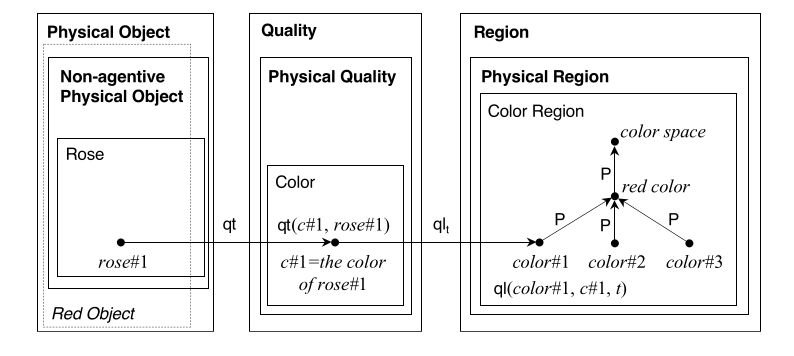
\includegraphics[scale=0.45]{01/poqr.png}
    \caption{Rappresentazione del colore di una rosa.}
\end{figure}

